\documentclass[a4paper]{article}
\usepackage[a4paper, total={6in, 8in}]{geometry}
\usepackage{float}

\usepackage{amsmath}
\usepackage{amssymb}
\usepackage{graphicx}
\usepackage{inputenc}
\usepackage{hyperref}
\usepackage{listings}
\usepackage{polski}
\usepackage{tcolorbox}

\title{Analiza ofert pracy w IT w Polsce w 2024 roku.}
\author{Łukasz Fabia (272724) \\ MSiD Lab 09:15 TP \\ Informatyka Stosowana}
\date{\today}

\begin{document}

\maketitle
\tableofcontents

\newpage

\section{Wstęp}

\quad Celem badań jest analiza danych dotyczących ofert pracy w IT. W swojej pracy postaram się
odpowiedzieć na pytanie, które umiejętności w branży IT są najbardziej poszukiwane oraz jakie jest wynagrodzenie,
w zależności od znajomości danych języków, frameworków czy narzędzi. W tym celu stworzę model, który będzie przewidywał stawki wynagrodzenia w zależności od danych wejściowych,
o których później.


\section{Dane}

\quad Dane pozyskam z serwisu \href{https://justjoin.it/}{justjoin.it}, który zbiera oferty pracy z wielu różnych stron internetowych. Na wyżej wymienionej stronie mamy katergorie, które mogą być przydatne do filtrowania danych. Są on mało jednak mało przydatne, ponieważ przypisane do ofert, nawiązują w jakiś sposób do np. JS. Katergorie są następujące:
JS, PHP, Ruby, Python, Java, Net, Mobile, C, DevOps, Security, Data, Go, Game, Scala. Moje dane będą pozyskiwane z tych podstron.\\
\quad Przeanalizuję zarobki tylko na b2b oraz zarobki na podstawie umowy o prace (uop). Są to najbardziej popularne formy zatrudnienia w IT. Umów takich jak zlecenie, umowa o staż pratykcznie nie występują. Do analizy będę również brał pod uwagę inne parametry, które występują w ofercie.

\textbf{\newline Technologia} - język programowania, framework, narzędzie, które jest wymagane w ofercie pracy.

\subsection{Model danej}
\quad Dane będą zawierały informacje o ofertach pracy, takie jak:
\begin{itemize}
    \item tytuł oferty,
    \item widełki dla B2B,
    \item widełki dla UOP,
    \item technologie dotyczące umowy,
    \item lokalizacja,
    \item doświadczenie: \textbf{junior, mid, senior},
    \item typ pracy: \textbf{stacjonarnie, hybrydowo, zdalnie.}
\end{itemize}

\subsection{Obsługa technologii, lokalizacji}

\quad Najpierw zdefiniuję słownik - klucz, wartość, gdzie klucz to ustandaryzowana technologia, a wartość do synonimy tej technologii.

\textit{np. : \ "JavaScript": [
"javascript",
"js",
"node.js",
"nodejs",
"express.js",
"expressjs",
].}

\quad Celem tego zabiegu jest zmniejszenie liczby technologii, które będę brał pod uwagę. Kolejnym
krokiem będzie obsługa lokalizacji. W tym przypadku, jeśli oferta dotyczy kilku miast, to po przetworzeniu pojawi się w zbiorze
klika ofert z tymi samymi danymi, ale dla różnych miast. Podobnie obsłużę kontrakty, które są w ofercie pracy, ponieważ z punktu
prawnego, jeśli oferta dotyczy obu kontraktów to tak naprawdę są to dwie różne oferty pracy.


\subsection{Pozykiwanie danych}

\quad Skorzystam z narzędzi do web scrappingu, w moim przypadku będzie
to \texttt{Selenium}, ponieważ strona ma dynamicznie ładowany content.\\


\textbf{Kroki:}

\begin{itemize}
    \item napisanie skryptu pobierającego linki do ofert pracy z danej kategorii, ponieważ nie chcemy śmiecowych ofert typu Product manager,
    \item napisanie skryptu przetwarzającego linki do ofert pracy, aby pobrać dane z oferty,
    \item przekierowanie wyniku do pliku json,
    \item normalizacja oraz oczyszczanie danych, kodowanie technologii do wektora przy pomocy MultiLabelBinarizer z \texttt{sklearn},
    \item kodowanie zmiennych kategorycznych (np. miasta, typ pracy, kontrakty),
    \item wzięcie średniej zarobków, a następnie usunięcie widełek w zarobkach (np. 10-15k $\implies$ 12.5k),
    \item rozbicie ofert pracy dla kontraktów oraz miast, np. mamy ofertę dla miasta A i B obie mają podane
          zarobki na b2b i uop, więc powstaną 4 nowe oferty, czyli A\_uop, A\_b2b, B\_uop, B\_b2b,
    \item usunięcie outlinerów,
    \item usunięcie tytułów ofert.
\end{itemize}

\begin{center}
    \textit{Ofert ze stawką godzinową było kilka, więc nie wpływają one na wyniki.}
\end{center}

\newpage

\section{Wygląd do danych}

\textit{uwaga przykładowe dane nie zawierają wszystkich kolumn bo jest ich za dużo, wszystkie dane można znaleźć w ../data/jobs.csv}


\textbf{Przykładowe dane:}

\begin{table}[H]
    \centering
    \begin{tabular}{|l|l|l|l|l|l|l|l|}
        \hline
        \textbf{avg\_salary} & \textbf{con\_code} & \textbf{loc\_code} & \textbf{exp\_code} & \textbf{mode\_code} & \textbf{AWS} & \dots & \textbf{android} \\ \hline
        23000.0              & 1                  & 50                 & 2                  & 0                   & 1            & \dots & 0                \\ \hline
        21742.5              & 1                  & 37                 & 2                  & 2                   & 0            & \dots & 0                \\ \hline
        21742.5              & 1                  & 17                 & 2                  & 2                   & 0            & \dots & 0                \\ \hline
        21742.5              & 1                  & 50                 & 2                  & 2                   & 0            & \dots & 0                \\ \hline
        21742.5              & 1                  & 54                 & 2                  & 2                   & 0            & \dots & 0                \\ \hline
    \end{tabular}
    \caption{Klika pierwszych wierszy moich danych.}
\end{table}



\begin{center}
    \begin{tcolorbox}[colback=white,colframe=blue, title=Uwaga]
        Skróciłem trochę nazwy, ponieważ musiałbym rozbijać tabele na kilka co byłoby mniej czytelne.
        \begin{enumerate}
            \raggedright
            \item con\_code - kod kontraktu
            \item loc\_code - kod lokalizacji
            \item exp\_code - kod doświadczenia
            \item mode\_code - kod typ pracy
        \end{enumerate}
    \end{tcolorbox}
\end{center}


\newpage

\section{Rozkłady i statystyki}

\quad Aktualnie w zbiorze \textit{jobs.csv} znajduje się \textbf{5696} ofert pracy, które będą poddane
analizie. Wszystkie dane są znormalizowane i gotowe do analizy. Analizę można zacząć od średniej zarobków
dla kontraktu B2B oraz UOP.


\textbf{Widełki dla Juniora: }

\begin{table}[H]
    \centering
    \begin{tabular}{|c|c|c|c|}
        \hline
        \textbf{PLN}     & \textbf{B2B} & \textbf{UOP} \\ \hline
        \textbf{średnia} & 9902.18      & 11057.05     \\ \hline
        \textbf{min}     & 5200.00      & 5500.00      \\ \hline
        \textbf{max}     & 16100.00     & 19000.00     \\ \hline
    \end{tabular}
    \caption{Średnie zarobki w PLN dla \texttt{juniora} w Polsce}
\end{table}

\textbf{Widełki dla Mida: }

\begin{table}[H]
    \centering
    \begin{tabular}{|c|c|c|c|}
        \hline
        \textbf{PLN}     & \textbf{B2B} & \textbf{UOP} \\ \hline
        \textbf{średnia} & 18025.50     & 15210.38     \\ \hline
        \textbf{min}     & 3132.50      & 6000.00      \\ \hline
        \textbf{max}     & 32500.00     & 27500.00     \\ \hline
    \end{tabular}
    \caption{Średnie zarobki w PLN dla \texttt{mida} w Polsce}
\end{table}

\textbf{Widełki dla Seniora: }

\begin{table}[H]
    \centering
    \begin{tabular}{|c|c|c|c|}
        \hline
        \textbf{PLN}     & \textbf{B2B} & \textbf{UOP} \\ \hline
        \textbf{średnia} & 25425.51     & 21734.47     \\ \hline
        \textbf{min}     & 9791.00      & 10000.00     \\ \hline
        \textbf{max}     & 40000.00     & 39040.50     \\ \hline
    \end{tabular}
    \caption{Średnie zarobki w PLN dla \texttt{seniora} w Polsce}
\end{table}

\quad Wynagrodzenia te są na dobrym poziomie, ponieważ dla Mida i Seniora mamy większą pensję na b2b niż na uop, dla juniora jest na odwrót. Przyczyną może być to, że umowę o pracę dostają bardzo dobrzy programiści albo jest mało ofert pracy dla juniora na b2b.


\newpage
\subsection{Jak się pracuje w IT?}

\begin{figure}[H]
    \centering
    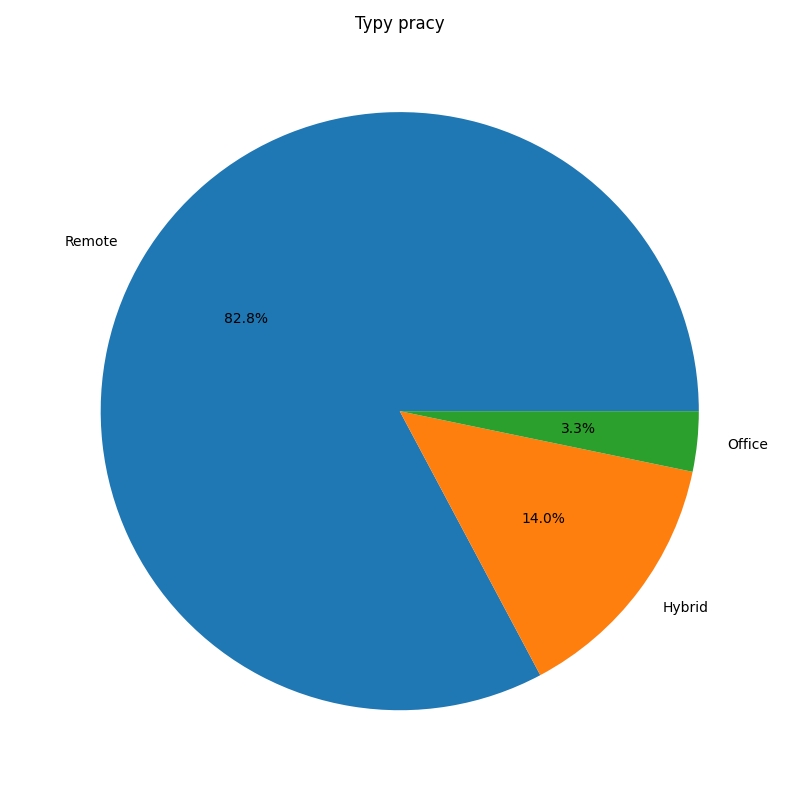
\includegraphics[width=\textwidth]{../analysis/plots/rozkłady/typy_pracy.png}
    \caption{Rozkład typów pracy}
\end{figure}

\quad Najwięcej ofert dotyczy pracy zdalnej.


\subsection{Kogo szukają pracodawcy?}

\begin{figure}[H]
    \centering
    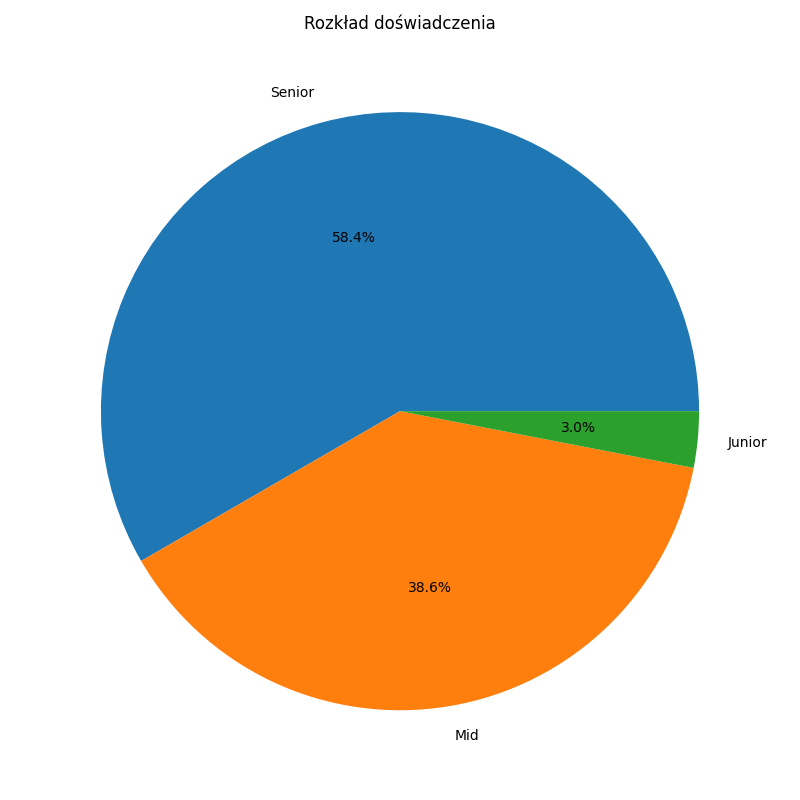
\includegraphics[width=0.8\textwidth]{../analysis/plots/rozkłady/rozkład_doświadczenia.png}
    \caption{Rozkład typów pracy}
\end{figure}

\quad Tak jak można było się spodziewać - najwięcej ofert pracy jest dla seniorów. Pracodawca ma większe zaufanie do Seniora/Mida. Gorzej jest z ofertami dla młodych programistów.
Tutaj ilość ofert wyniósła zaledwie 159. W porównianiu do innych grup jest to niewiele.

\begin{center}
    \textit{Czy to oznacza, że młodzi programiści mają trudniej, a słynne "eldorado" w IT jest tylko dla doświadczonych programistów?}
\end{center}

\quad Można stwierdzić, że juniorzy mają trudniejszy start w branży IT, ale jeśli im się uda, to zarobki są atrakcyjne.


\subsection{Jak rozkładają się zarobki?}

\begin{figure}[H]
    \centering
    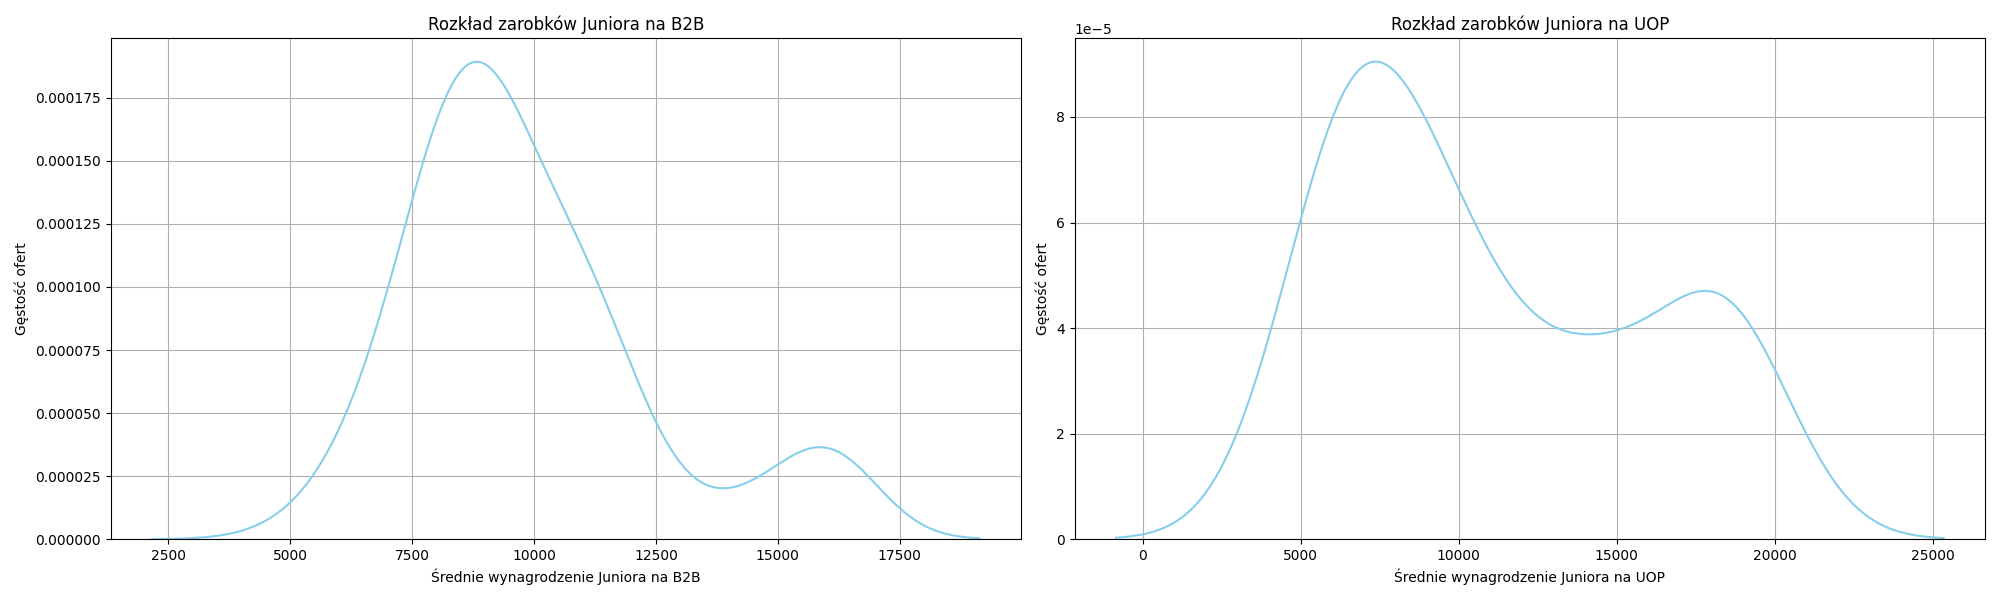
\includegraphics[width=0.8\textwidth]{../analysis/plots/rozkłady/pensje_dla_juniora.png}
    \caption{Rozkłady zarobków dla poszczególnych umów dla juniorów}
\end{figure}

\begin{figure}[H]
    \centering
    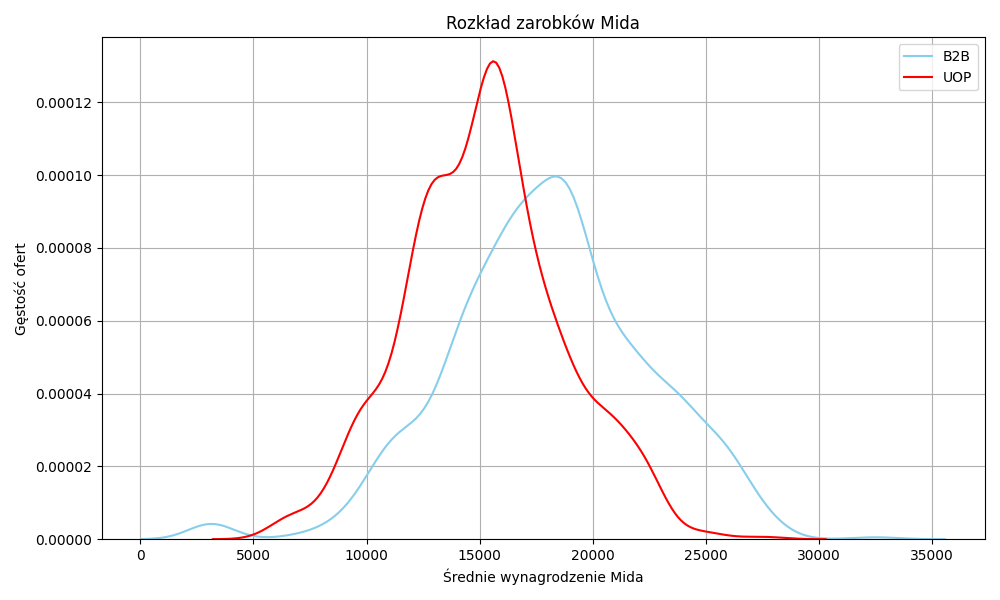
\includegraphics[width=0.8\textwidth]{../analysis/plots/rozkłady/pensje_dla_mida.png}
    \caption{Rozkłady zarobków dla poszczególnych umów dla midów}
\end{figure}

\begin{figure}[H]
    \centering
    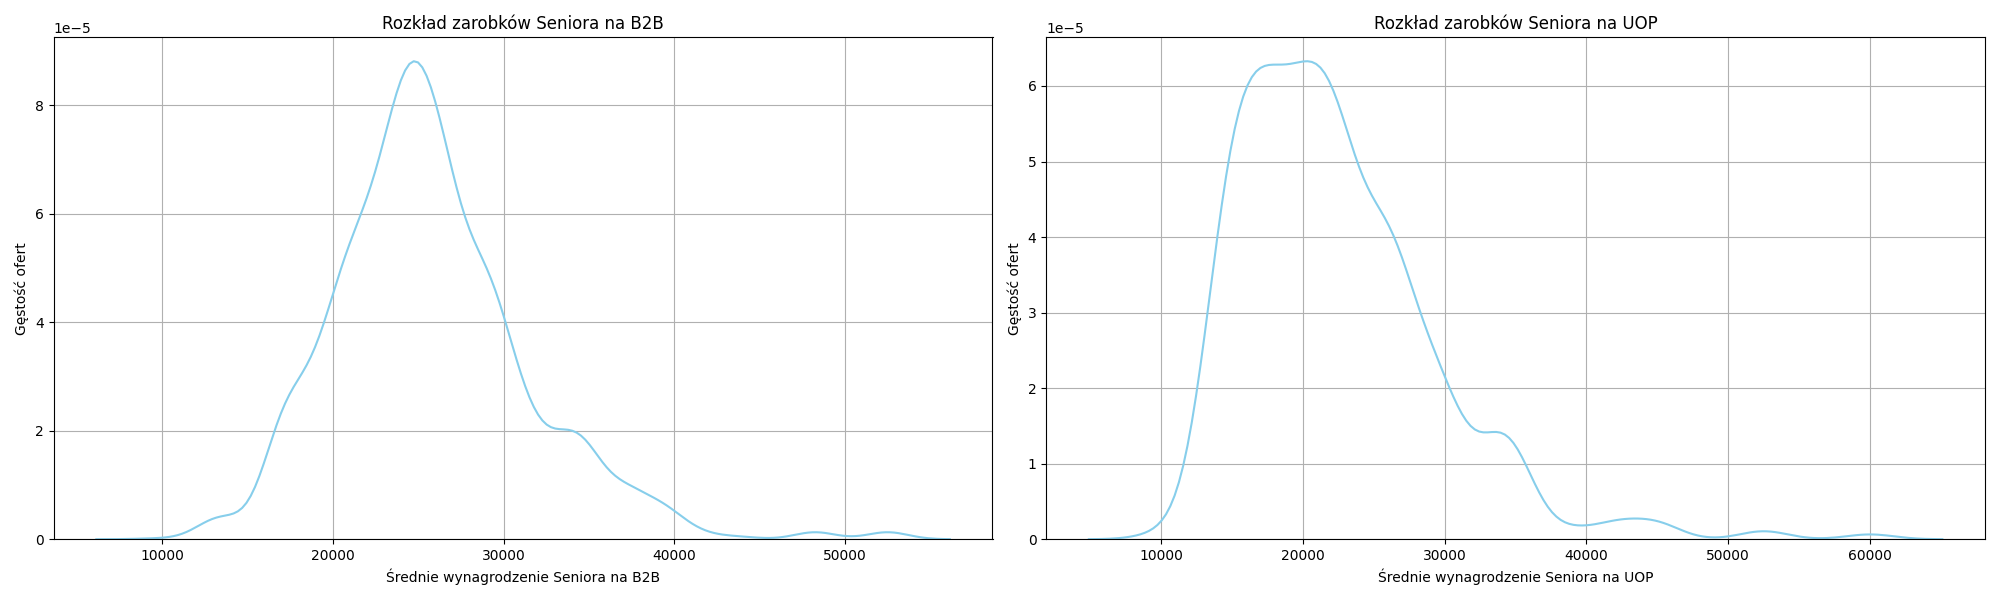
\includegraphics[width=0.8\textwidth]{../analysis/plots/rozkłady/pensje_dla_seniora.png}
    \caption{Rozkłady zarobków dla poszczególnych umów dla seniorów}
\end{figure}

\quad Można zauważyć, że rozkłady przypominają rozkłady normalne, chociaż dla juniorów pensje na uop
są bardziej wypłaszczone, co znaczy, że zarobki są bardziej zróżnicowane lub było zbyt mało ofert dla juniorów a oferty ze zbioru miały skrajne widełki na umowie o pracę. Dla seniorów zarobki na b2b są bardziej skupione wokół średniej.


\subsection{Jakie technologie są najbardziej poszukiwane?}

\begin{figure}[H]
    \centering
    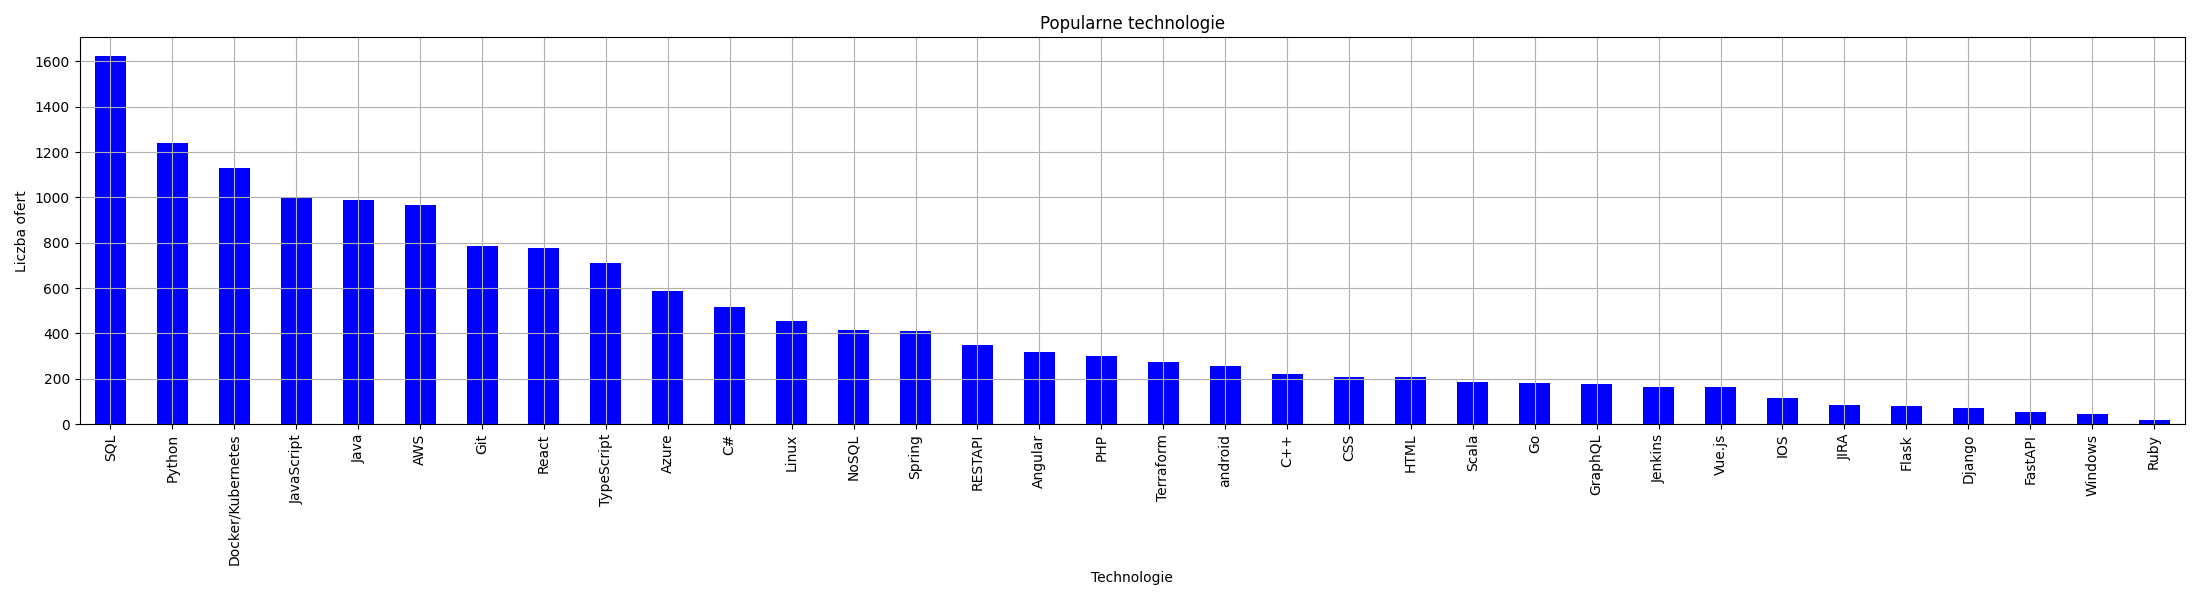
\includegraphics[width=\textwidth]{../analysis/plots/rozkłady/popularne_technologie.png}
    \caption{Popularne technologie w ofertach pracy w Polsce}
\end{figure}

\quad Najpopularniejszą technologią okazał się \texttt{SQL}. Bez jego znajomości trudno znaleźć pracę w IT. Oczywiście nie mogło zabraknąć \texttt{Pythona} oraz \texttt{JavaScriptu}, jeśli chodzi o języki skryptowe.
Co warto, zazanczyć narzędzia takie jak \texttt{Docker} czy \texttt{Kubernetes} również są bardzo popularne i warto je znać. \texttt{Java} wygrywa z \texttt{C\#}.

\subsection{Gdzie jest największy popyt na programistów?}

\begin{figure}[H]
    \centering
    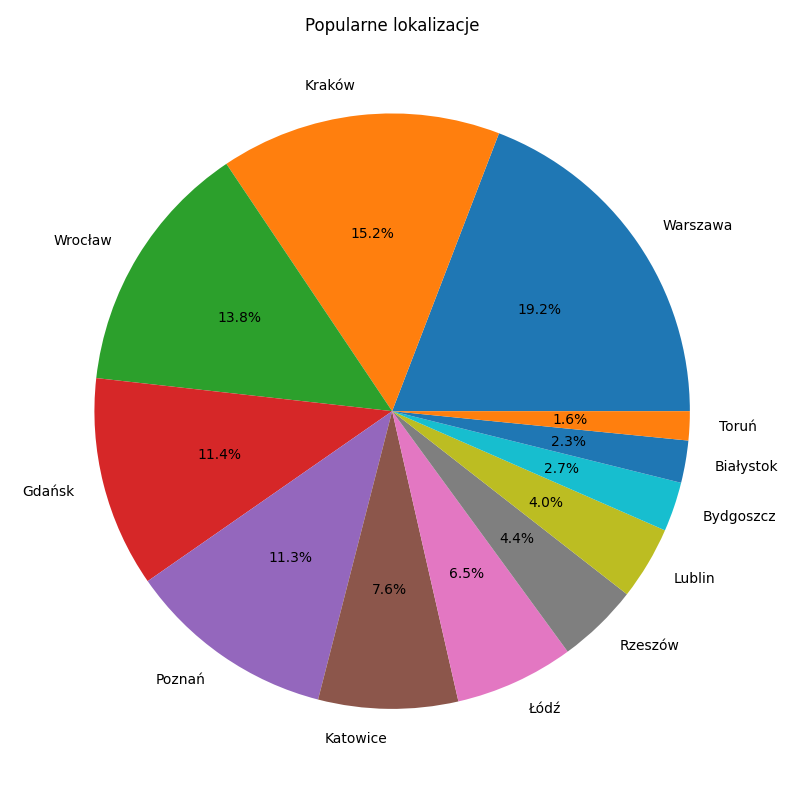
\includegraphics[width=0.8\textwidth]{../analysis/plots/rozkłady/popularne_lokalizacje.png}
    \caption{Popularne miasta w ofertach pracy w Polsce}
\end{figure}

\quad Zestawienie miast jest zgodne z oczekiwaniami, najwięcej ofert pracy jest kolejno w: \textbf{Warszawie}, \textbf{Krakowie} oraz \textbf{Wrocławiu}, chociaż w
\textbf{Gdańsku} również pojawiawiły się stosunkowo duże ilości ofert pracy.


\subsection{Gdzie poszukiwani są juniorzy?}

\begin{figure}[H]
    \centering
    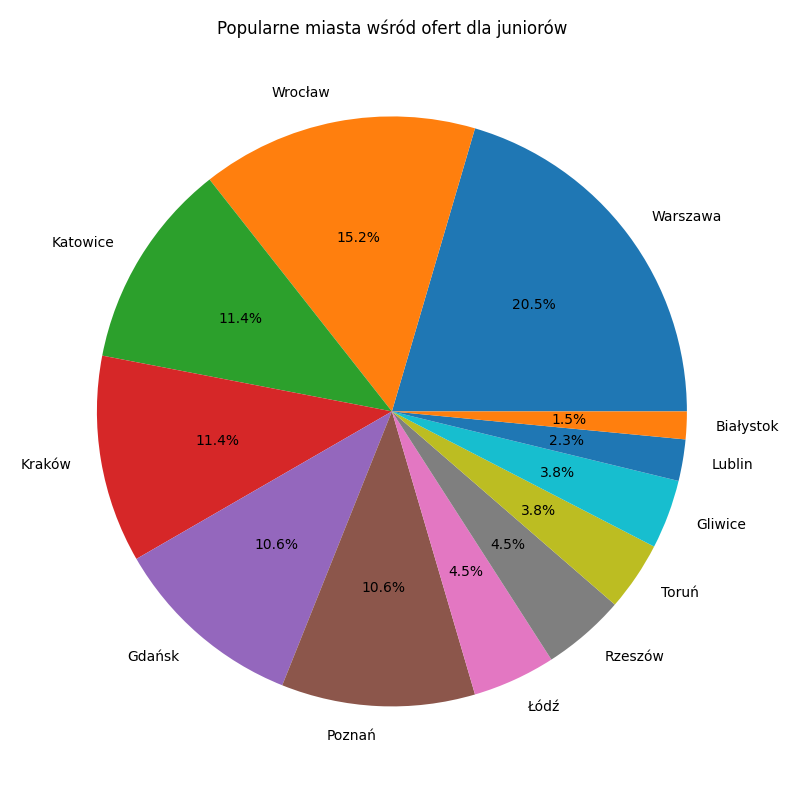
\includegraphics[width=\textwidth]{../analysis/plots/rozkłady/popularne_miasta_wśród_ofert_dla_juniorów.png}
    \caption{Popularne miasta w ofertach dla juniorów}
\end{figure}

\quad \textbf{Warszawa} jest najbardziej przyjazna dla juniorów, ale
warto zauważyć, że wykres nie różni się bardzo od poprzedniego. Jednak, to \textbf{Gdańsk} jest na 3 miejscu w zestawieniu dla juniorów.

\section{Powiązania między danymi}

\subsection{Powiązania między technologiami}

\begin{figure}[H]
    \centering
    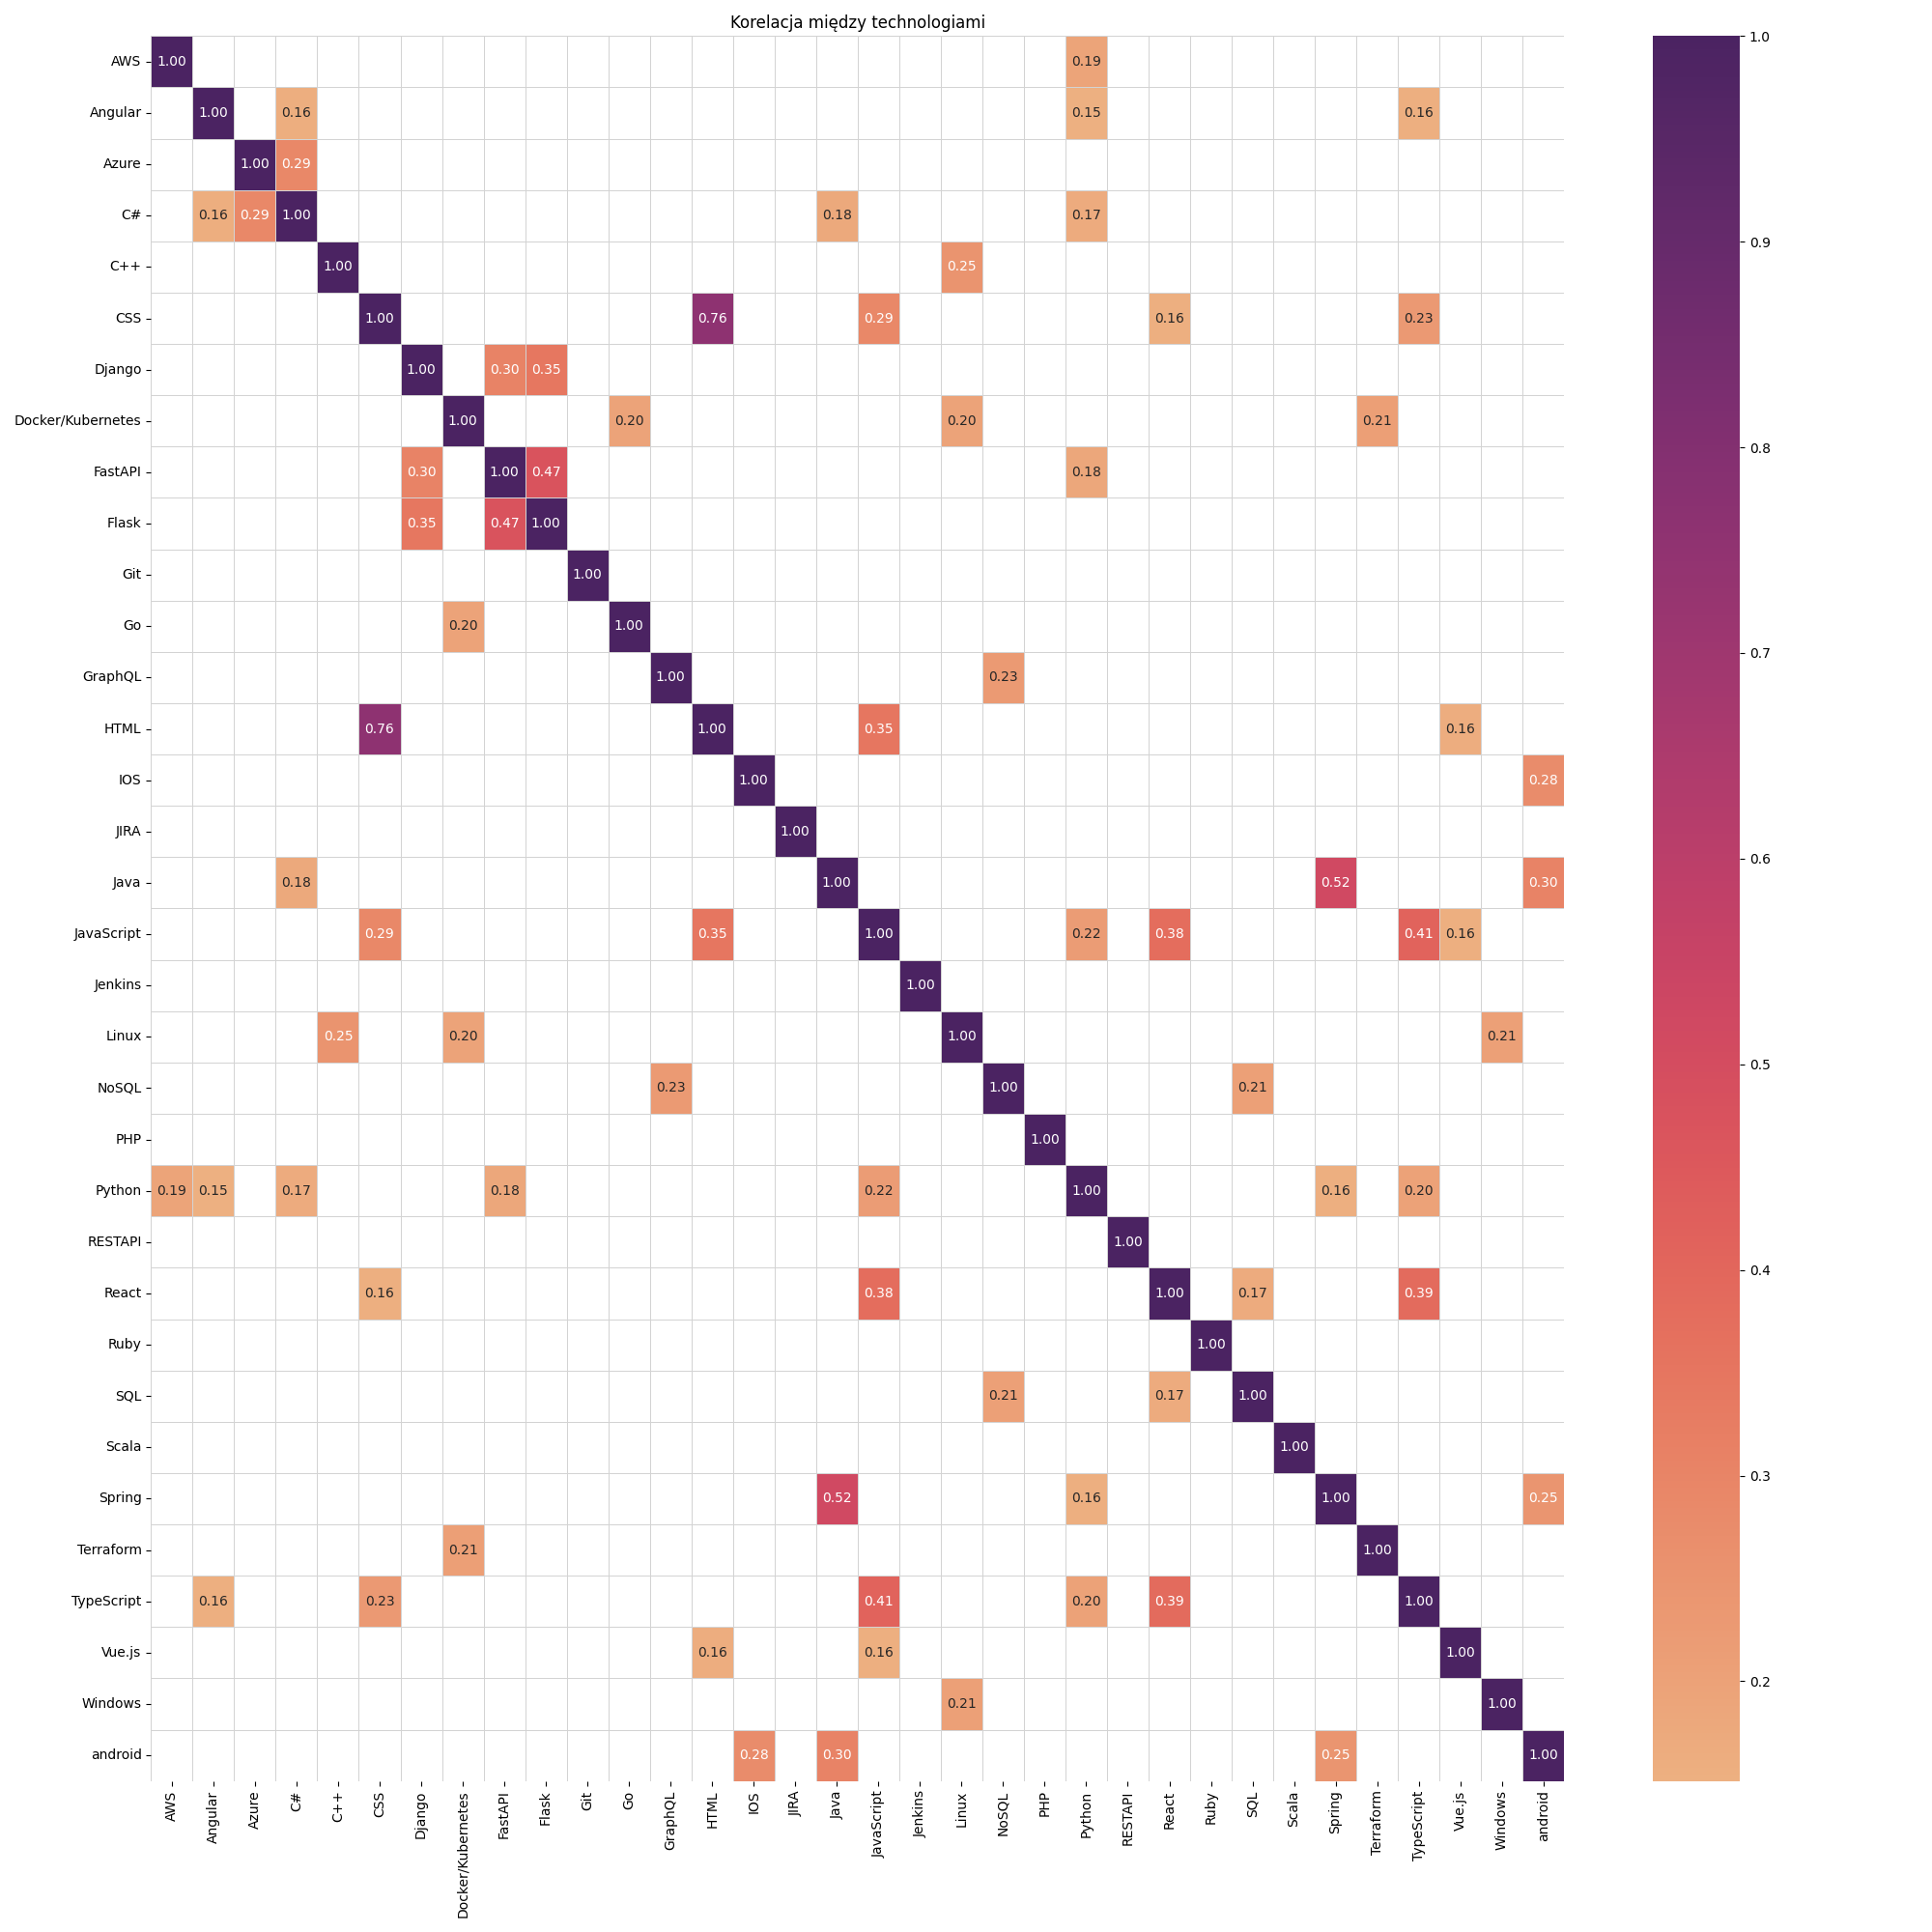
\includegraphics[width=\textwidth]{../analysis/plots/korelacje/korelacja_między_technologiami.png}
    \caption{Powiązania między technologiami, zawierająca tylko wartości korelacji większe niż 0.14}
\end{figure}

\quad \textbf{Co można zauważyć?}

\begin{enumerate}
    \item HTML i CSS idą ze prawie w parze - co jest zrozumiałe, bo to podstawy frontendu.
    \item Przy Javie warto znać Springa.
    \item React i JS i TS często pojawiają sie razem w ofertach pracy obok HTML i CSS.
    \item Ucząc się Django to warto znać inne frameworki backendowe takie jak Flask czy FastAPI.
    \item Interesując się Embedded'em warto znać C/C++ oraz Linux.
    \item Technologie microsoftu takie jak C\#, Azure występują razem.
\end{enumerate}

\quad To tylko kilka przykładów wynikających z wykresu powyżej, ale warto zauważyć, że nie ma tu silnych powiązań między technologiami. Oferty pracy są zróznicowane i zależą od firmy.


\subsection{Powiązania między innymi zmiennymi}

\begin{figure}[H]
    \centering
    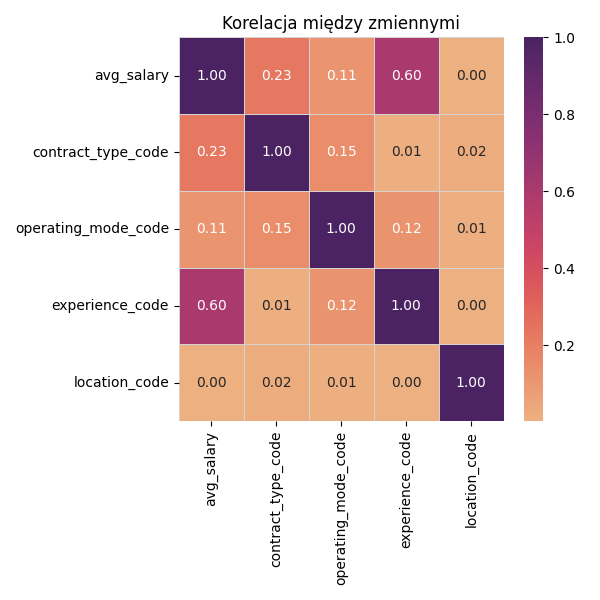
\includegraphics[width=\textwidth]{../analysis/plots/korelacje/korelacja_między_zmiennymi.png}
    \caption{Powiązania między innymi zmiennymi}
\end{figure}

\quad \textbf{Co można zauważyć?}

\begin{enumerate}
    \item Średnia pensja jest mocno powiązana z doświadczeniem.
    \item Typ kontraktu zależy od doświadczenia.
\end{enumerate}


\subsection{Zarobek a technologie}

\begin{figure}[H]
    \centering
    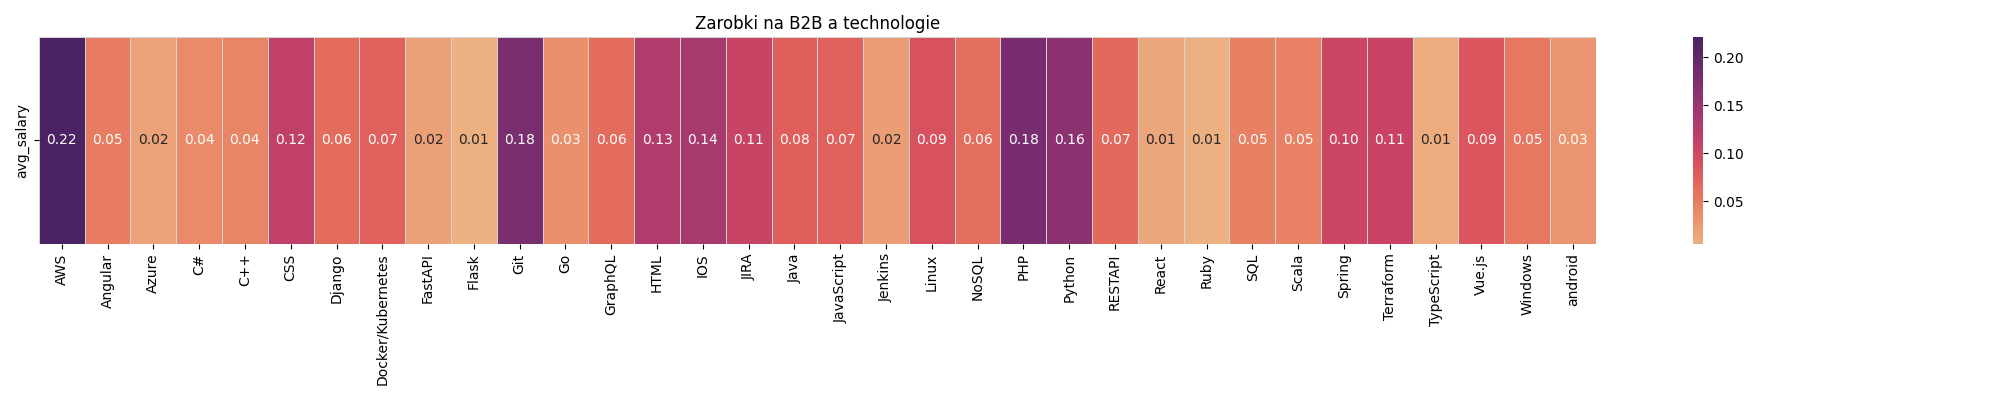
\includegraphics[width=\textwidth]{../analysis/plots/korelacje/zarobki_na_b2b_a_technologie.png}
    \caption{Powiązania między zarobkiem b2b a technologiami}
\end{figure}

\quad AWS, Git, Python, PHP mają wypłw na pensję na b2b, ale nie jest on duży.

\begin{figure}[H]
    \centering
    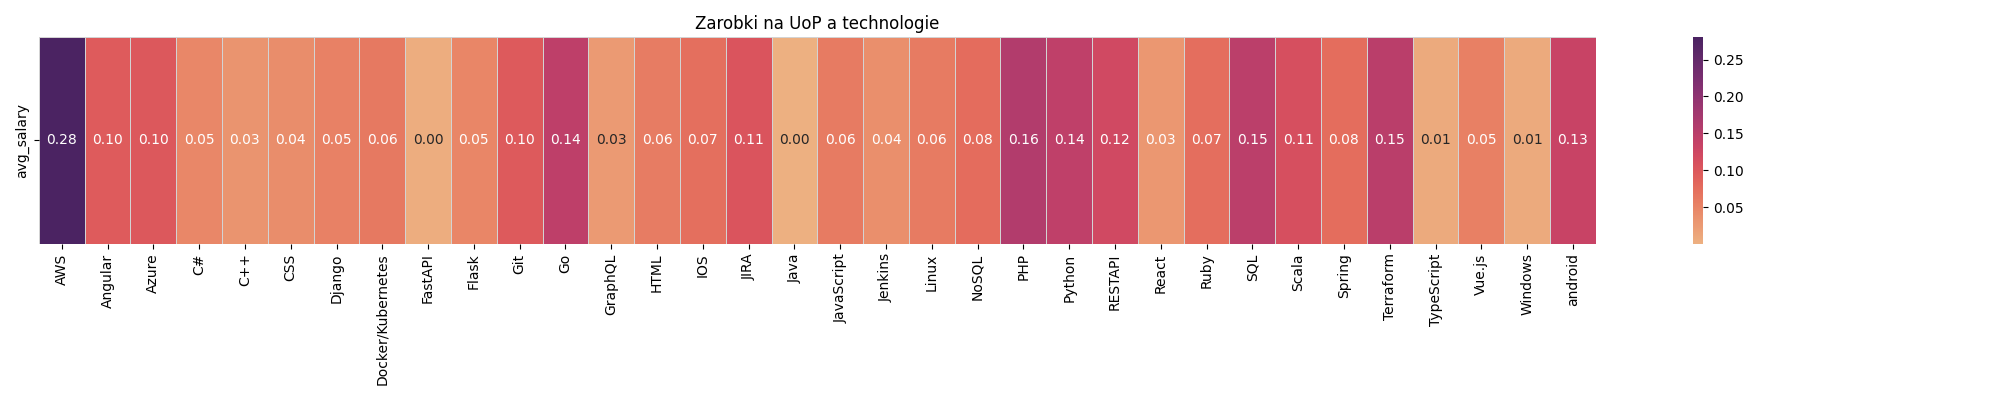
\includegraphics[width=\textwidth]{../analysis/plots/korelacje/zarobki_na_uop_a_technologie.png}
    \caption{Powiązania między zarobkiem uop a technologiami}
\end{figure}

\quad PHP, Python, AWS, SQL, Go, Terraform mają wpływ na pensję na uop, ale nie jest on duży.


\section{Czy da się przewidzieć zarobki, w zależności od mojego tech-stacku?}

\subsection{Ogólnie o problemie}

\quad \textbf{Oczywiście}, że tak, da się przewiedzieć zarobki od tech-stacku. Kiedy mamy dane to możemy nauczyć model, który na wejściu dostanie zmienne i przewidzi dla nas
zarobki. Dokładniej mówiąc, model otrzyma na wejściu dane takie jak:

\texttt{Input:}

\begin{itemize}
    \item tech-stack,
    \item lokalizacja,
    \item typ pracy,
    \item doświadczenie,
    \item typ kontraktu (B2B, UoP).
\end{itemize}

\texttt{Output:}

\begin{itemize}
    \item Zarobki w PLN.
\end{itemize}


\subsection{Dobór modeli}

\quad Modele, które będą wykorzystane w analizie to:

\begin{enumerate}
    \item Regresja liniowa:
          \begin{itemize}
              \item \texttt{LinearRegression}
              \item \texttt{Ridge}
              \item \texttt{Lasso}
          \end{itemize}
    \item \texttt{DecisionTreeRegressor}
    \item \texttt{RandomForestRegressor}
\end{enumerate}

\textit{Wszyskie modele pochodzą z modułu \href{https://scikit-learn.org/stable/}{skelearn}.}

\subsection{Trochę statystyki - metryki}

\quad Do oceny modeli wykorzystam metryki takie jak:

\begin{itemize}
    \item \textbf{Root Mean Squared Error} - pierwiastek z średniego błędu kwadratowego,
    \item \textbf{R-squared} - współczynnik determinacji $R^2$,
    \item \textbf{Mean Absolute Error} - średni błąd bezwzględny,
\end{itemize}

\quad ale wybrać będę po RMSE.

\subsubsection{Pierwiastek ze średniego błędu kwadratowego}

\quad \textbf{Root Mean Squared Error (RMSE)} - to pierwiastek z MSE, daje nam miarę błędu przewidywań w tych samych jednostkach co dane wejściowe.
Można go interpretować jako średnią oczekiwaną różnicę +/- między wartością przewidywaną a rzeczywistą \cite{rmse}.

\begin{equation}
    RMSE = \sqrt{\frac{1}{n} \sum_{i=1}^{n} (y_i - \hat{y_i})^2}
\end{equation}

\subsubsection{Współczynnik determinacji}

\quad \textbf{R-squared (R2)} - to miara oceny dopasowania funkcji regresji do danych. Wartość bliska 1 oznacza, że funkcja regresji lepiej dopasowała sie do danych.

\begin{equation} R^2=1-\frac{\sum({y_i}-\hat{y_i})^2}{\sum(y_i-\bar{y})^2}, R^2 \in [0, 1] \end{equation}

\subsubsection{Średni błąd bezwzględny}

\quad \textbf{Mean Absolute Error (MAE)} - to średni bezwzględny błąd między przewidywaniami a rzeczywistymi wartościami.
Jest bardziej odporny na wartości odstające niż RMSE (outlinery), ponieważ nie podnosi błędów do kwadratu.

\begin{equation}
    {\displaystyle \mathrm {MAE} ={\frac {\sum _{i=1}^{n}\left|y_{i}-x_{i}\right|}{n}}.}
\end{equation}


\subsection{Jak to zrobię?}

\quad Moje rozwiązanie problemu opiera się na wybraniu modeli regresji liniowej, drzewa decyzyjnego oraz lasu losowego, które będą
tuningowane za pomocą \texttt{GridSearchCV} w celu znalezienia najlepszych hiperparametrów. Wyniki są dostępne w folderze
\texttt{../analysis/models\_tuning.csv}. Kolejnym krokiem jest przeprowadzenie uczenia modeli i wybranie najlepszego
na podstawie RMSE. Następnie przewidzę zarobki dla kilku danych wejściowych, a na końcu przedstawię wyniki w postaci wizualizacji.\\

\begin{abstract}
    \quad W następnych rodziałach skupię się na wynikach modeli, a także na wizualizacji wyników, aby nie
    tworzyć zbyt długiego raportu, nie będe analizować słabych modeli tylko skupię się na dwóch najlepszych. Wszyskie wyniki z uczenia zostaną zapisane w folderze \texttt{../analysis/plots/wyniki/} ew. można też podejrzeć plik z rozwiązaniem problemu w \texttt{../analysis/analysis.ipynb}.

    \quad Stosowane podziałki to 80:20, czyli 80\% danych do uczenia, a 20\% do testowania modelu oraz 60:40.
\end{abstract}

\subsubsection{Wyniki dla podziału danych 80:20}

\begin{table}[H]
    \centering
    \begin{tabular}{|c|c|c|c|}
        \hline
        \textbf{Model}        & \textbf{Mean Absolute Error} & \textbf{Root Mean Squared Error} & \textbf{R\textsuperscript{2} Score} \\ \hline
        LinearRegression      & 3485.34                      & 4371.01                          & 0.56                                \\ \hline
        DecisionTreeRegressor & 2367.30                      & 3469.85                          & 0.72                                \\ \hline
        RandomForestRegressor & 1529.31                      & 2757.87                          & 0.82                                \\ \hline
        Ridge                 & 3485.97                      & 4374.60                          & 0.56                                \\ \hline
        Lasso                 & 3484.26                      & 4371.90                          & 0.56                                \\ \hline
    \end{tabular}
\end{table}


\quad Łatwo zauważyć, że najlepszym modelem jest \texttt{RandomForestRegressor}, który ma
najniższe wartości błędów oraz najwyższy współczynnik determinacji, kolejnym
będzie \texttt{DecisionTreeRegressor}, choć nie jest on idealny powiedziałbym, słaby.
Pozostałe modele, czyli modele regresji liniowej mają pratykcznie te same wyniki.

\begin{figure}[H]
    \centering
    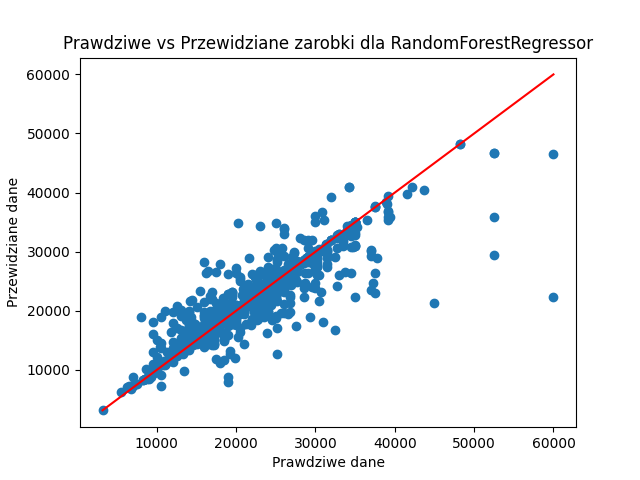
\includegraphics[width=\textwidth]{../analysis/plots/wyniki/0.8&0.2/RandomForestRegressor/scatter.png}
    \caption{Dopasowanie danych przewidzianych do prawdziwych}
\end{figure}

\begin{figure}[H]
    \centering
    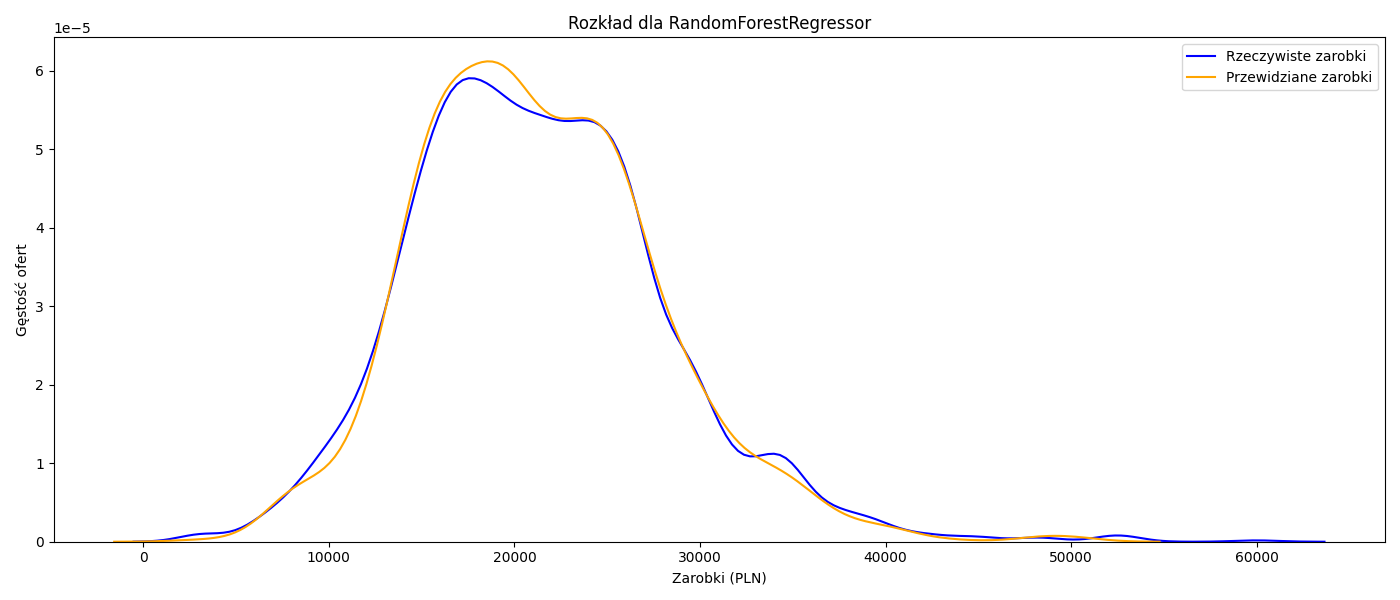
\includegraphics[width=\textwidth]{../analysis/plots/wyniki/0.8&0.2/RandomForestRegressor/salary_dist.png}
    \caption{Rozkład dla przewidzianych i prawdziwych wartości}
\end{figure}

\begin{figure}[H]
    \centering
    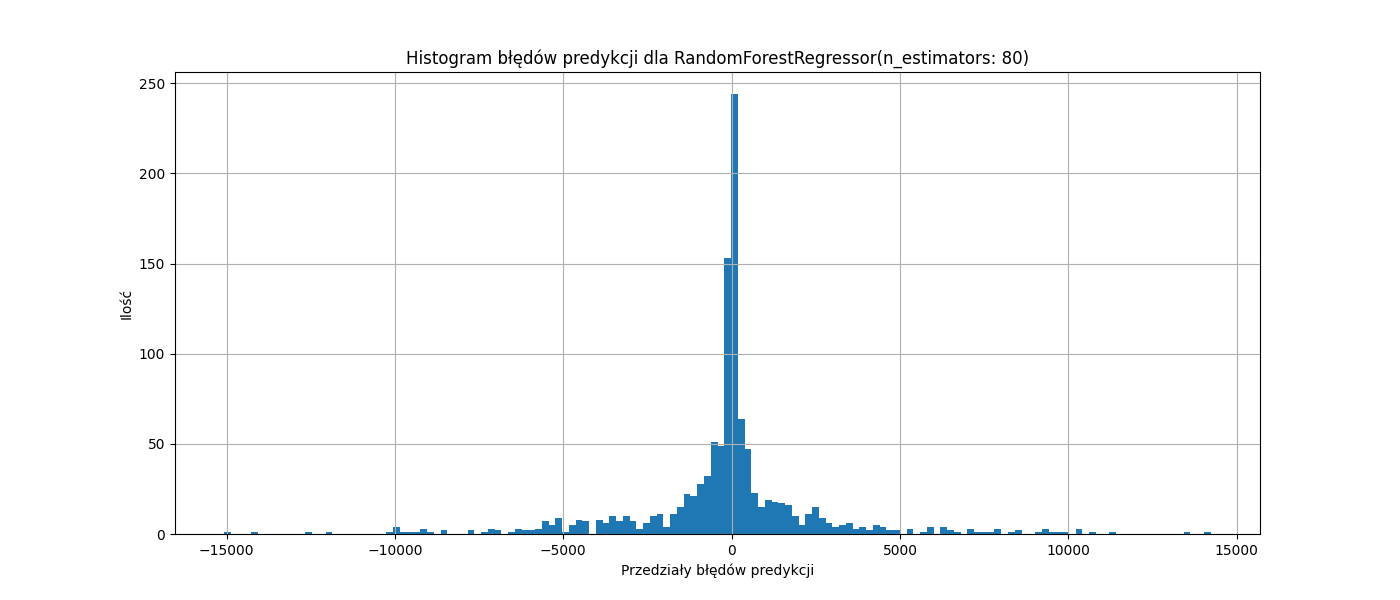
\includegraphics[width=\textwidth]{../analysis/plots/wyniki/0.8&0.2/RandomForestRegressor/errors.png}
    \caption{Rozkład dla przewidzianych i prawdziwych wartości}
\end{figure}

\begin{figure}[H]
    \centering
    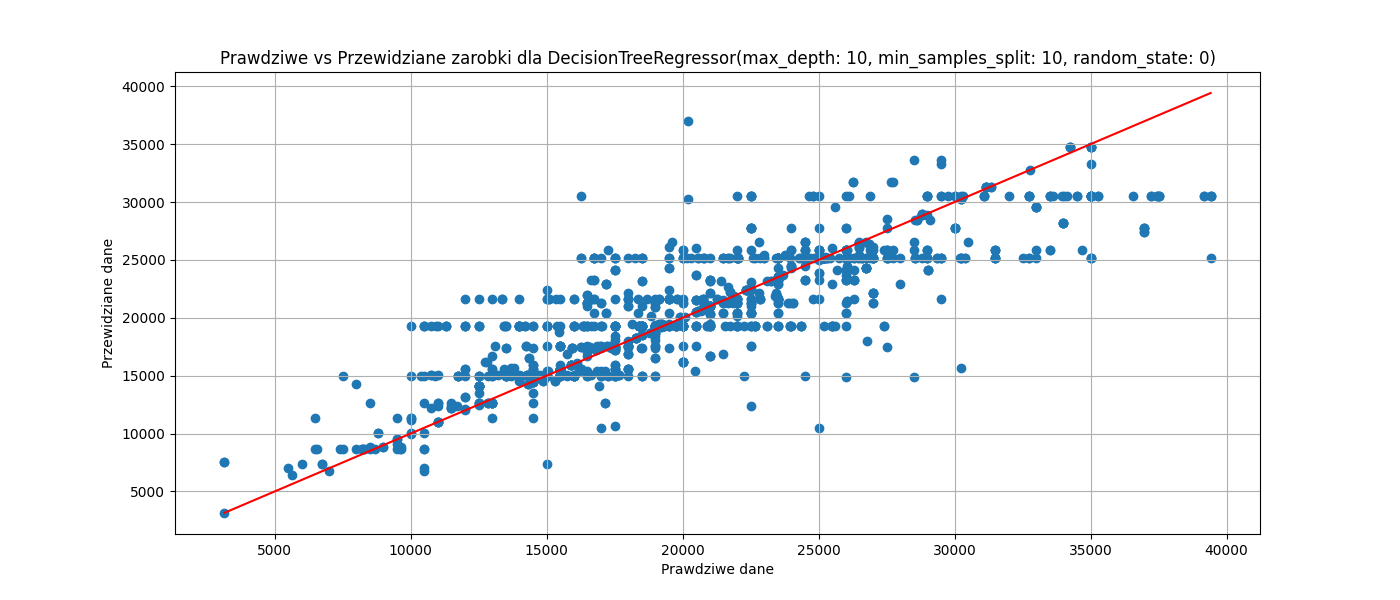
\includegraphics[width=\textwidth]{../analysis/plots/wyniki/0.8&0.2/DecisionTreeRegressor/scatter.png}
    \caption{Dopasowanie danych przewidzianych do prawdziwych}
\end{figure}

\begin{figure}[H]
    \centering
    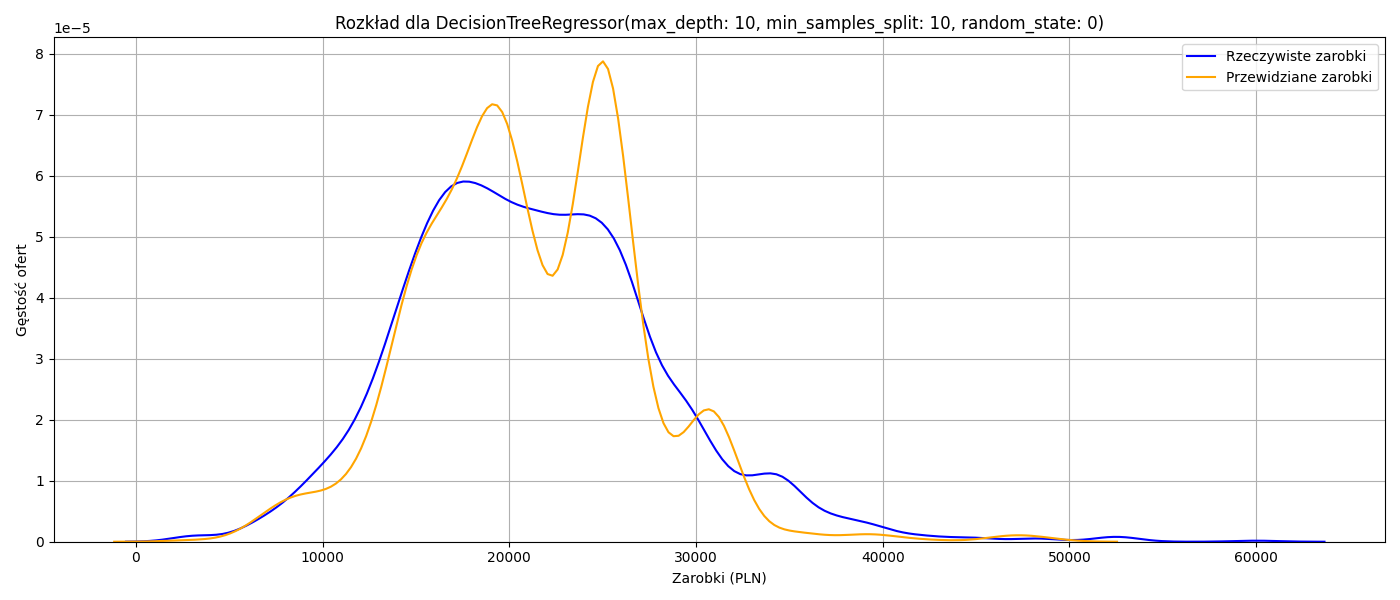
\includegraphics[width=\textwidth]{../analysis/plots/wyniki/0.8&0.2/DecisionTreeRegressor/salary_dist.png}
    \caption{Rozkład dla przewidzianych i prawdziwych wartości}
\end{figure}

\begin{figure}[H]
    \centering
    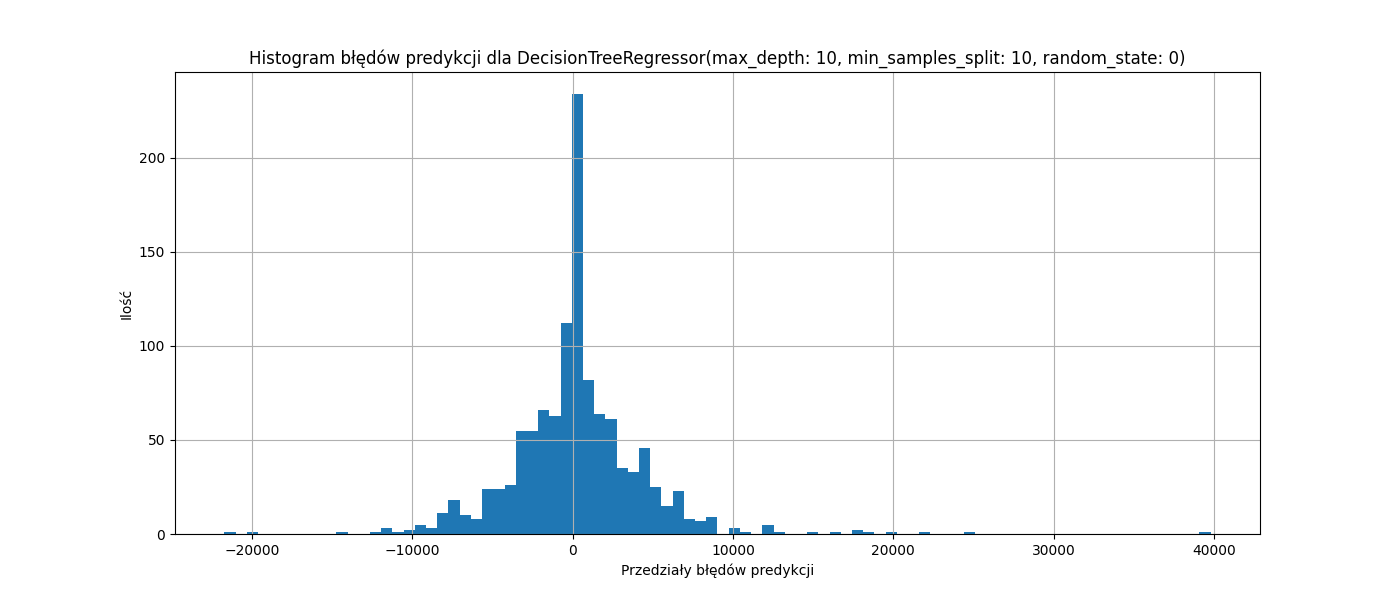
\includegraphics[width=\textwidth]{../analysis/plots/wyniki/0.8&0.2/DecisionTreeRegressor/errors.png}
    \caption{Rozkład dla przewidzianych i prawdziwych wartości}
\end{figure}

\subsubsection{Podsumowanie wyników dla 80:20}

\quad Wyniki pokazały nam, że najlepszym modelem do przewidywania zarobków jest \texttt{RandomForestRegressor} z parametrami \texttt{n\_estimators=80},
chociaż błędy były dość wysokie, ale może to wynikać z rozpiętości wiedełek pensji lub mogą być spowodowane małą ilością ofert pracy dla juniorów. Warto zauważyć, że
dla najlepszego modelu dane były w miarę skupione w prostej wyznaczającej idealny wynik. Dopasowanie rozkładu było też całkiem dobre, ponieważ
wykresy w większej części nachodziły na siebie. Histogramy były skupione wokół zera, co może oznaczać, że model dobrze przewiduje zarobki.


\subsubsection{Wyniki dla podziału danych 60:40}

\begin{table}[H]
    \centering
    \begin{tabular}{|c|c|c|c|}
        \hline
        \textbf{Model}        & \textbf{Mean Absolute Error} & \textbf{Root Mean Squared Error} & \textbf{R\textsuperscript{2} Score} \\ \hline
        LinearRegression      & 3455.46                      & 4312.71                          & 0.55                                \\ \hline
        DecisionTreeRegressor & 2477.46                      & 3586.54                          & 0.69                                \\ \hline
        RandomForestRegressor & 1720.41                      & 2912.11                          & 0.80                                \\ \hline
        Ridge                 & 3455.05                      & 4314.41                          & 0.55                                \\ \hline
        Lasso                 & 3454.5                       & 4314.37                          & 0.55                                \\ \hline
    \end{tabular}
\end{table}

\begin{figure}[H]
    \centering
    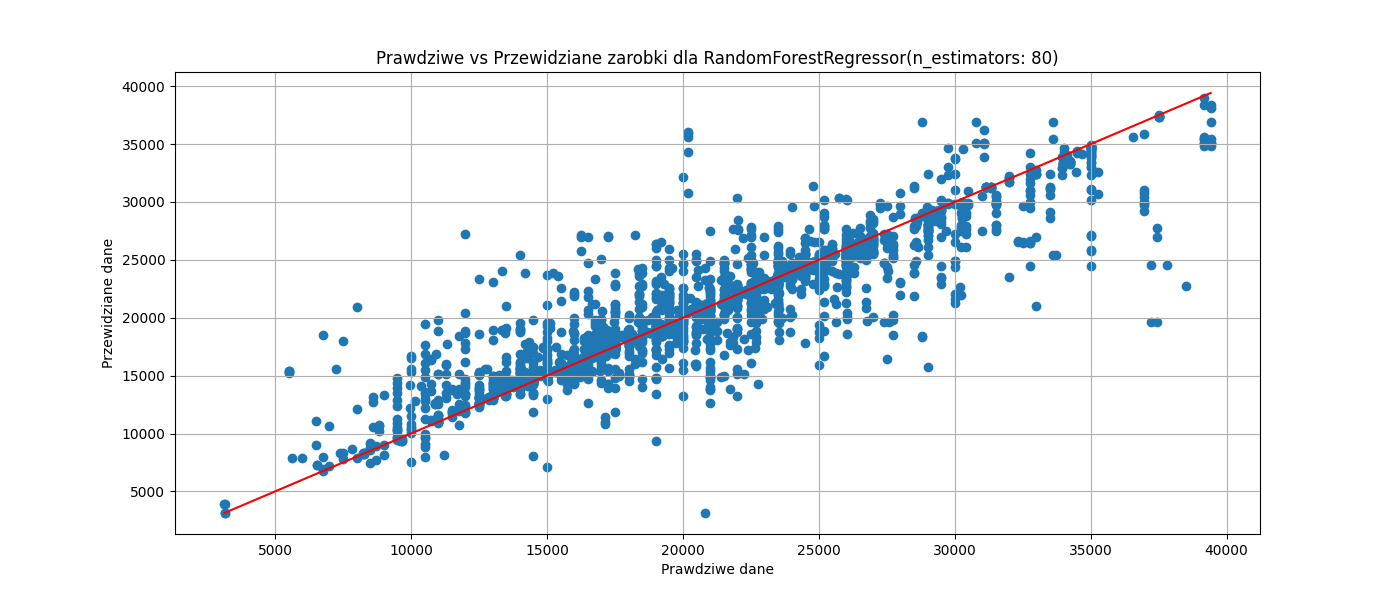
\includegraphics[width=\textwidth]{../analysis/plots/wyniki/0.6&0.4/RandomForestRegressor/scatter.png}
    \caption{Dopasowanie danych przewidzianych do prawdziwych}
\end{figure}

\begin{figure}[H]
    \centering
    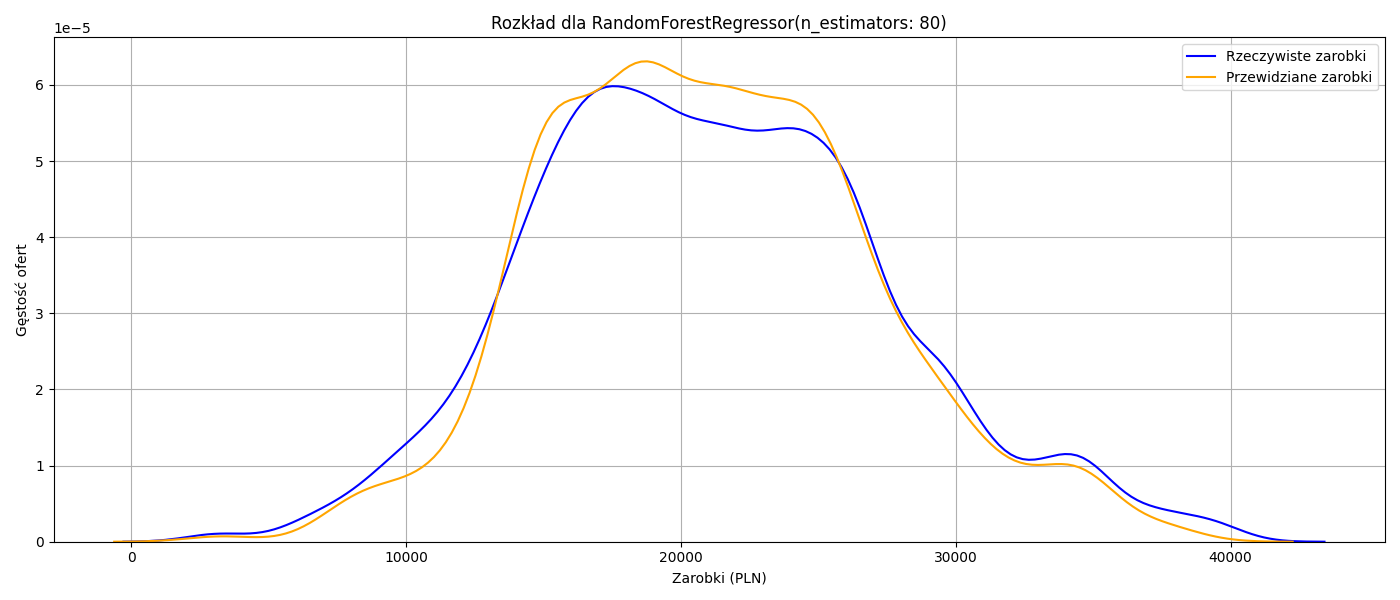
\includegraphics[width=\textwidth]{../analysis/plots/wyniki/0.6&0.4/RandomForestRegressor/salary_dist.png}
    \caption{Rozkład dla przewidzianych i prawdziwych wartości}
\end{figure}

\begin{figure}[H]
    \centering
    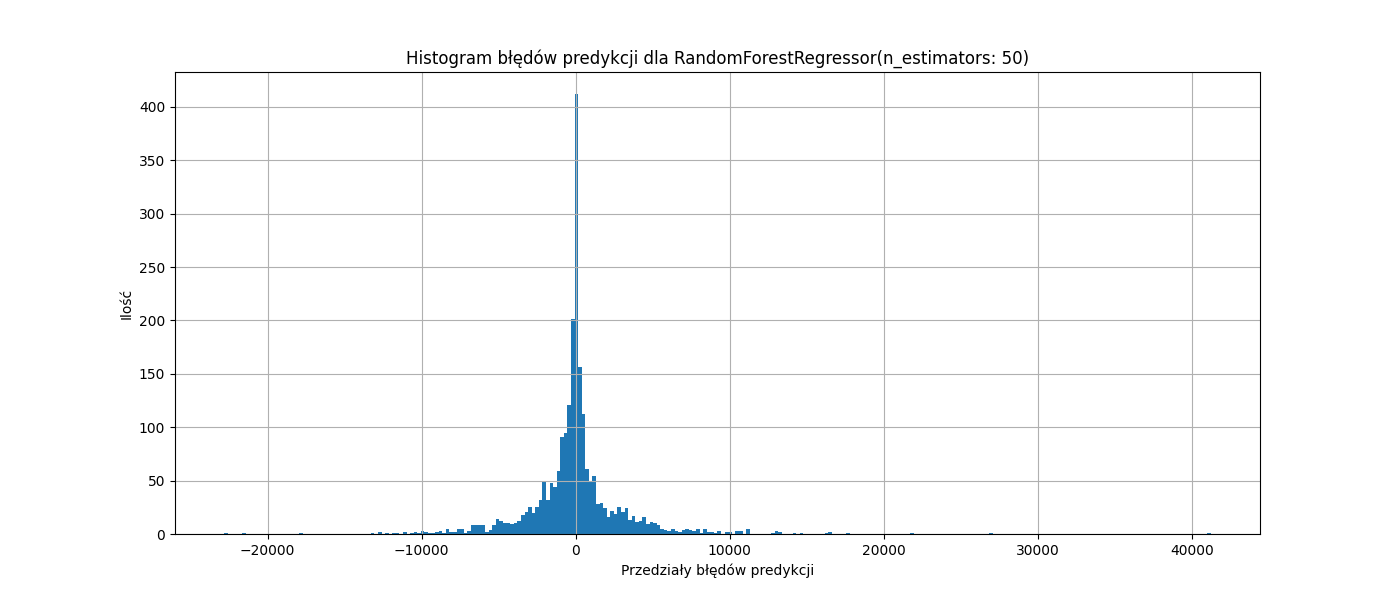
\includegraphics[width=\textwidth]{../analysis/plots/wyniki/0.6&0.4/RandomForestRegressor/errors.png}
    \caption{Rozkład dla przewidzianych i prawdziwych wartości}
\end{figure}

\begin{figure}[H]
    \centering
    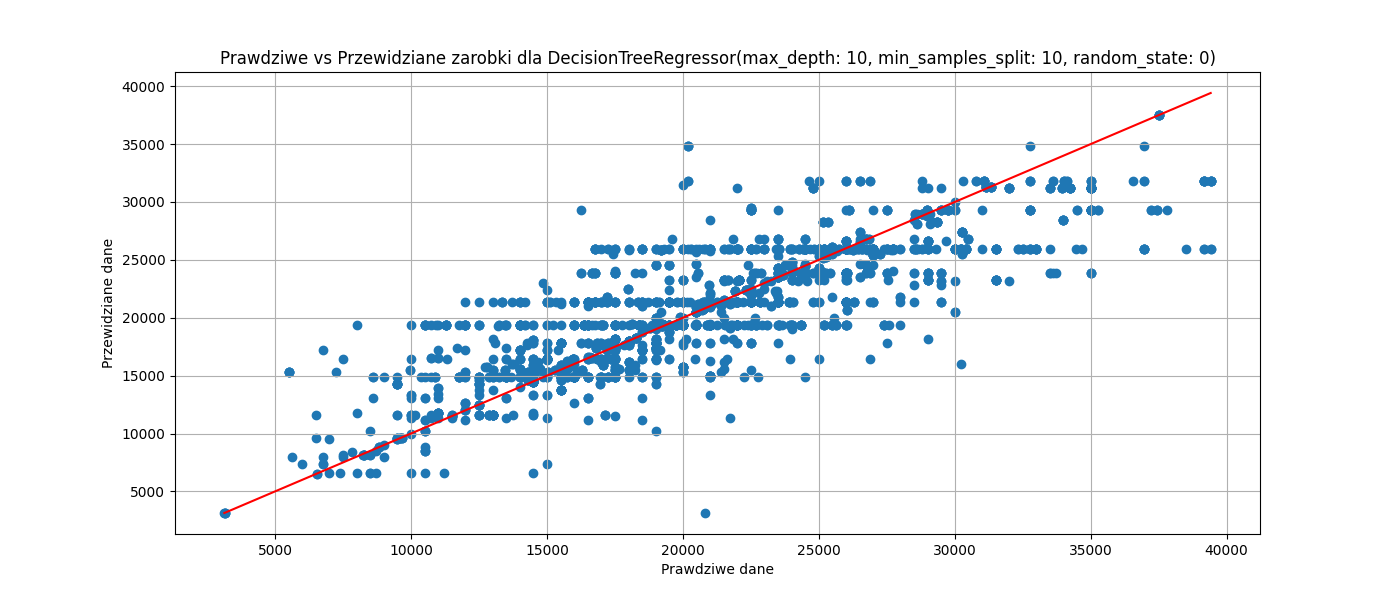
\includegraphics[width=\textwidth]{../analysis/plots/wyniki/0.6&0.4/DecisionTreeRegressor/scatter.png}
    \caption{Dopasowanie danych przewidzianych do prawdziwych}
\end{figure}

\begin{figure}[H]
    \centering
    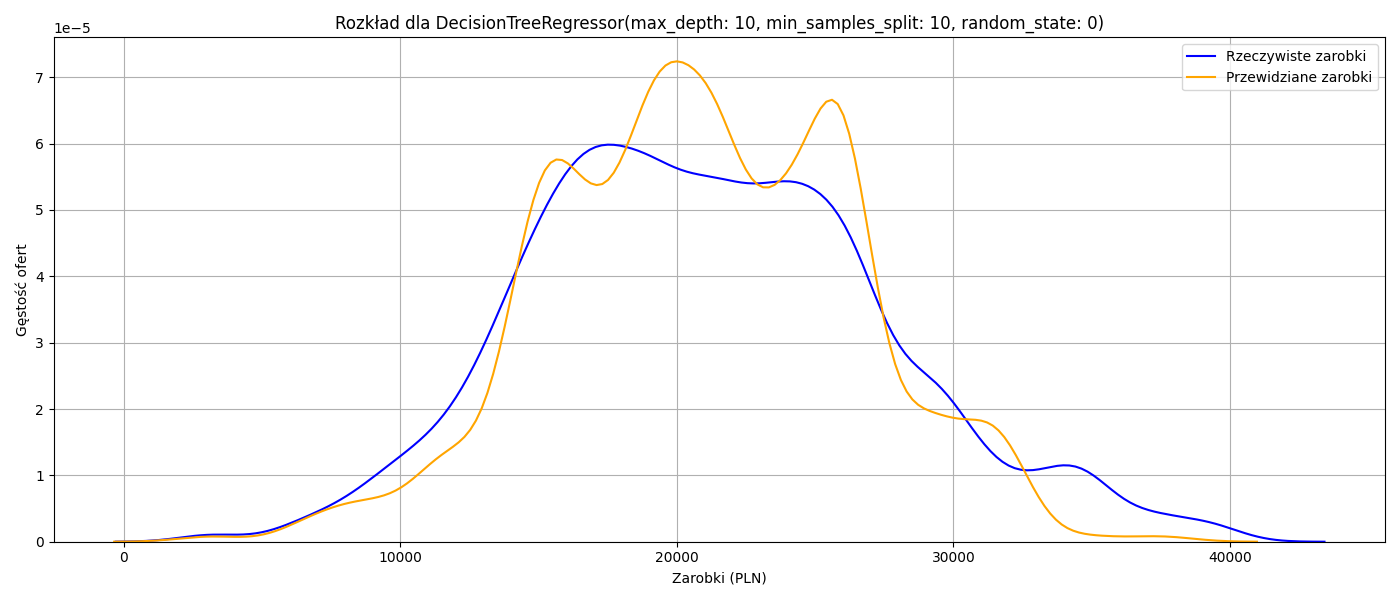
\includegraphics[width=\textwidth]{../analysis/plots/wyniki/0.6&0.4/DecisionTreeRegressor/salary_dist.png}
    \caption{Rozkład dla przewidzianych i prawdziwych wartości}
\end{figure}

\begin{figure}[H]
    \centering
    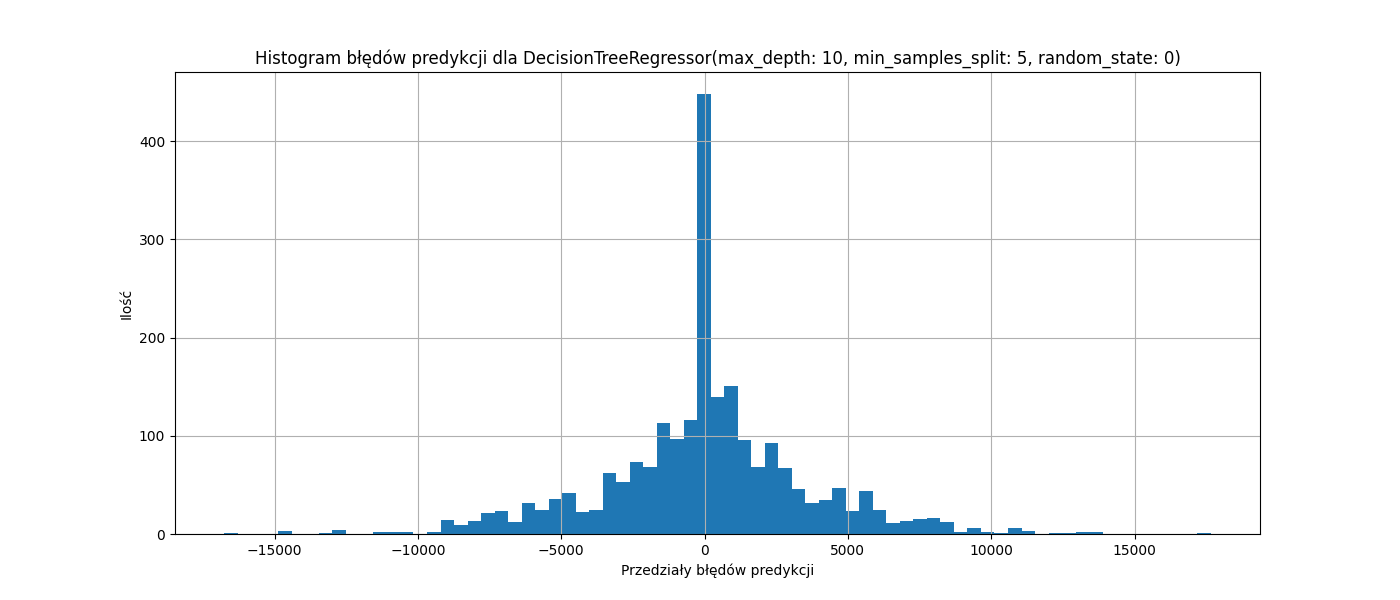
\includegraphics[width=\textwidth]{../analysis/plots/wyniki/0.6&0.4/DecisionTreeRegressor/errors.png}
    \caption{Rozkład dla przewidzianych i prawdziwych wartości}
\end{figure}

\subsubsection{Podsumowanie wyników dla 60:40}


\quad Wyniki są mniej precyzyjne niż dla poprzedniego testu, ale to wynika z faktu, że model uczył się na mniejszej
ilości ofert. Warto zauważyć, że najlepszy model to \texttt{RandomForestRegressor} z parametrami \texttt{n\_estimators=80},
potem był \texttt{DecisionTreeRegressor}, który miał gorsze wyniki niż w poprzednim teście. Warto zauważyć, że modele regresji liniowej osiągnęły lepsze wyniki jeśli chodzi o błędy, ale współczynnik determinacji był gorszy niż dla poprzedniego podziału.

\section{Podsumowanie}
\quad Najlepszym modelem będzie \texttt{RandomForestRegressor(n\_estimators=80)},
ponieważ dawał najmniejsze błędy chociaż i tak w skali zarobków nie były one małe.
Do uczenia modelu lepiej wybrać podziałkę 80:20. Wydaje mi się również, że aby uzyskać lepsze wyniki,
należałoby zaktualizować zbiór danych o nowe oferty (głównie oferty dla juniorów). Warto dodać, że
gdy kompilujemy skrypt to metryki mogą się różnić dla \texttt{RandomForestRegressor}, ale są to różnice rzędu 20-50 +/-, metryki. Może to wynikać z faktu jak dzielone są dane na treningowe i testowe.
Oczywiście, model może być jeszcze lepiej rozwinięty, jeśli dodane zostałby nowe cechy, np. stopień naukowy lub nowe technologie lub większe wyspecyfikowanie technologii.

\quad Podczas pracy również można było sporządzić wykres, który przedstawiał najważniejsze zmienne wypływające na wynagrodzenie.

\begin{figure}[H]
    \centering
    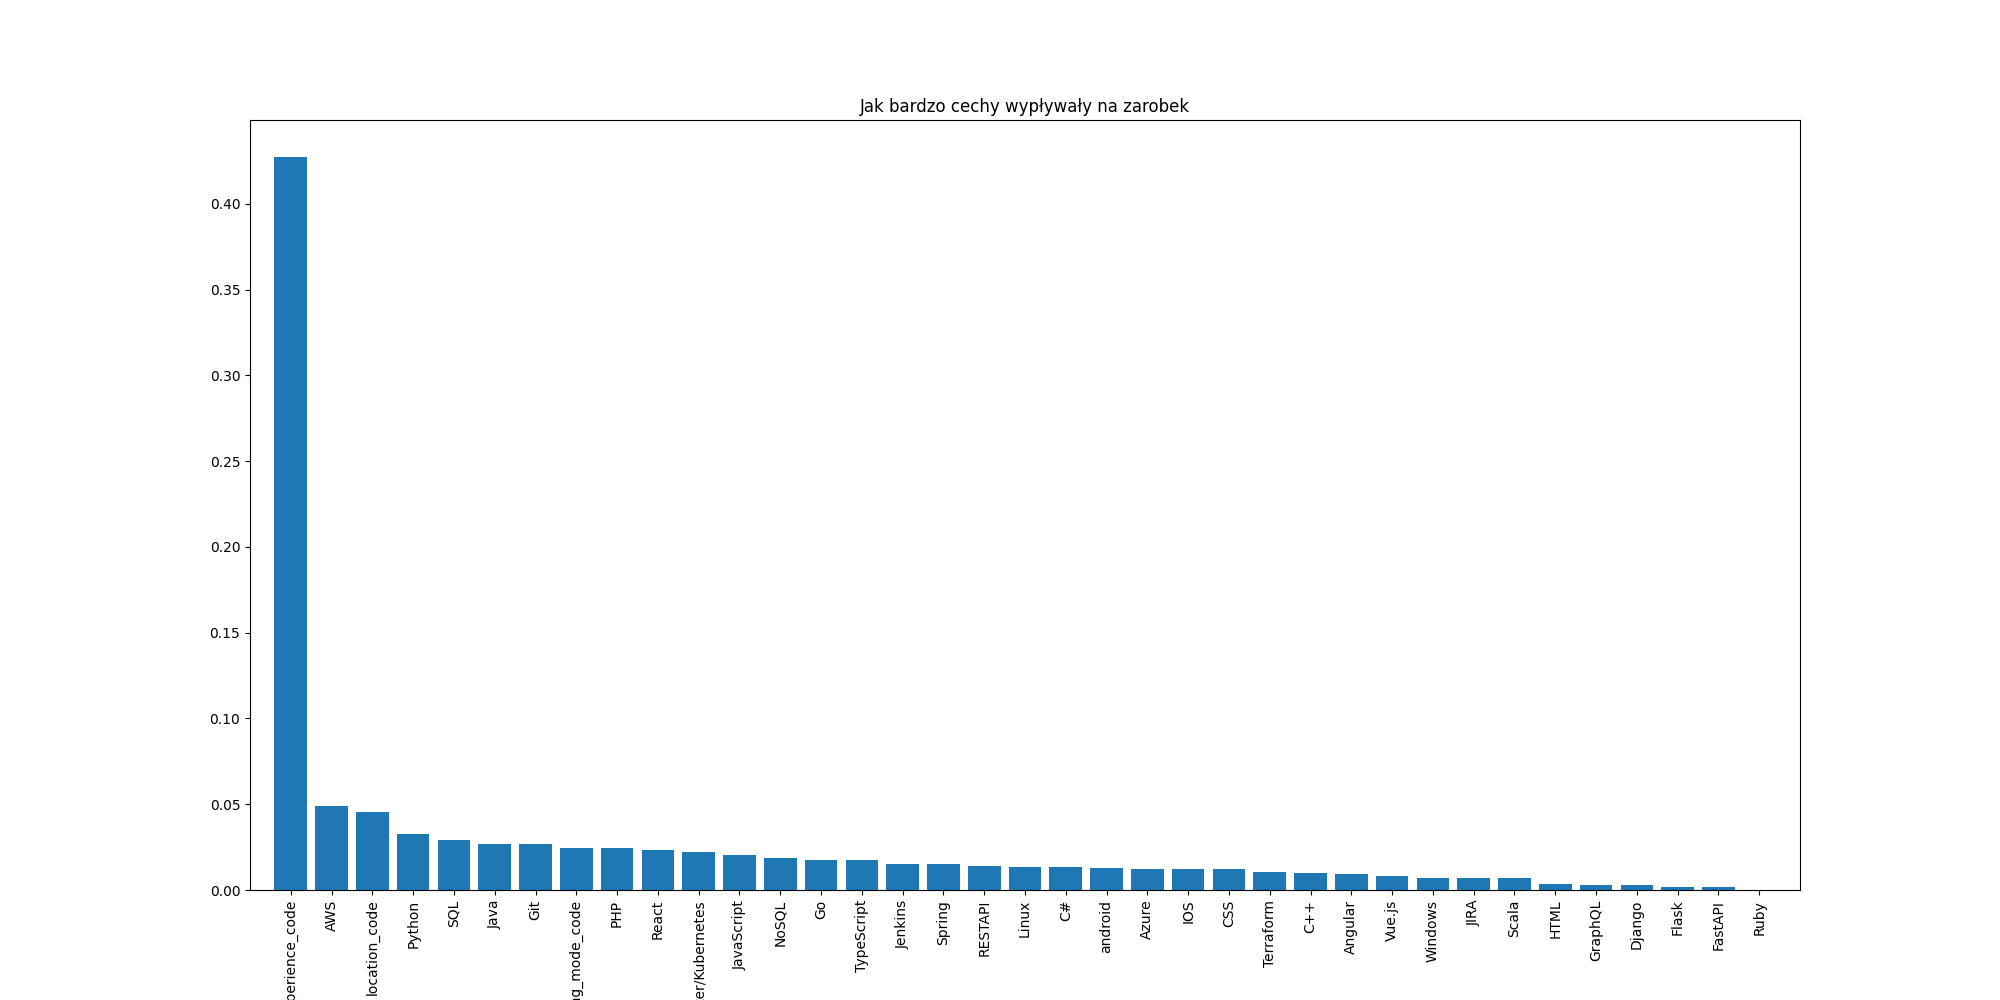
\includegraphics[width=\textwidth]{../analysis/plots/wyniki/importance_of_vars.png}
    \caption{Zmienne mające wypłw na wynagrodzenie w ofercie pracy}
\end{figure}

\quad Jak łatwo zauważyć, \textbf{doświadczenie} miało największy wpływ na przewidywaną wartość.
Kolejnymi zmiennymi, które miały wpływ to \textbf{typ umowy}, \textbf{miasto}, \textbf{AWS} czy \textbf{Python}.

\newpage

\section{Testowanie wyuczonego modelu}

\quad Tak jak już wcześniej wspomniałem model, który uznałem za odpowiedni, czyli popełniający najmniejszy błąd
spośród wszystkich to \texttt{RandoForestRegressor(n\_estimators=80)}, dla podziałki 80:20.
Przetestuję model, który przewidzi mi pensję na b2b i na umowie o pracę w zależności od technologii, które znam. Najważniejszą rzeczą jest tutaj to, żeby zarobki na b2b były większe niż na uopie,
ponieważ pracodawcy nie muszą ponosić kosztów dodatkowych podatków, składek i świadczeń \cite{uop_vs_b2b}.

\begin{itemize}
    \item \textbf{location}: Wrocław
    \item \textbf{exp}: Junior
    \item \textbf{operating\_mode}: Hybrid
    \item \textbf{tech\_stack}:
          \begin{itemize}
              \item Docker/Kubernetes
              \item Python
              \item React
              \item TypeScript
              \item JavaScript
              \item HTML/CSS
          \end{itemize}
\end{itemize}

\subsection{Wyniki testów}

\quad Pensja w lokalizacji \textbf{Wrocław} dla \textbf{Junior} znającego \textit{Docker/Kubernetes, Python, Linux, React, TypeScript, JavaScript}:

\begin{itemize}
    \item 8442.62 PLN Brutto na umowie o pracę,
    \item 9118.08 PLN Brutto na b2b
\end{itemize}

\textbf{Wnioski po analizie zaprezentowanych wyników:}

\begin{enumerate}
    \item Istotna jest konfiguracja technologii w procesie tworzenia modelu a nie jej ilość.
    \item Jeśli model dostał na treningu oferty z wysokimi zarobkami to wyniki będą trochę zawyżone.
    \item Rodzaj zastosowanej technologii ma wpływ na większe lub mniejsze wynagrodzenie.
\end{enumerate}

\quad Myślę, że udało mi się stworzyć przykładowy model przewidujący zarobki w zależności od innych
zmiennych w ofercie pracy. Wśród modeli ten okazał się mieć najmniej błędów, co jest
satysfakcjonujące, a przewidywane wartości są, powiedzmy jasno, sensowne.\\

\begin{center}
    \href{https://github.com/lukaszfabia/RaportIT}{\textit{Link to całego projektu znajduje się na moim \textbf{GitHubie}}}
\end{center}


\section{Bibliografia}

\begin{thebibliography}{9}
    \bibitem{uop_vs_b2b}
    \href{https://bizky.ai/blog/umowa-o-prace-a-kontrakt-b2b-co-sie-bardziej-oplaca/}{\textit{Umowa o pracę a kontrakt B2B – jak zarobisz więcej?}}, bizky.ai

    \bibitem{rmse}
    \href{https://help.qlik.com/pl-PL/cloud-services/Subsystems/Hub/Content/Sense_Hub/AutoML/scoring-regression.htm}{\textit{Ocena modeli regresji}}, qlik.com
\end{thebibliography}


\end{document}


